\documentclass[a4paper]{book}

\usepackage[ngerman]{babel}								%Sprache
\usepackage[ansinew]{inputenc}						%Umlaute ohne Maske
%\usepackage{amsmath}											%Mathe f�r alle!
%\usepackage{amsfonts}											%Mathefonts
\usepackage{graphicx}											%Bessere Grafikunterst�zung
\usepackage[pdfborder = 0 0 0]{hyperref}	%Nette PDFs ohne M�h...


\title{PPLT-Handbuch}
\author{Hannes Matuschek}
\date{2005-05-25}


\begin{document}
%	\begin{titlepage}
%		\maketitle
%		\vfill
%		\tableofcontents
%	\end{titlepage}
	\parindent = 0em
	\parskip = 2ex
	%\pagestyle{}
	
\chapter{Einf�hrung}
	\section{Was ist PPLT?}
	PPLT steht f�r \textit{Potsdamer Prozessleit-Technik} in Anlehnung an die 
	\textit{\index{Achener Prozessleittechnik}Achener Prozessleittechnik}
	\footnote{\href{http://www.acplt.de}{http://www.acplt.de}}. 
	Die PPLT ist ein so genanntes Framework, f�r die Kommunikation mit 
	Industriesteuerungen,	Sensoren, Aktoren oder mit 
	Haus-Auto\-matisierungs\-technik.

	Das System ist quelloffen und ist unter der \index{GNU-GPL} GNU-GPL bezeiungsweise der 
	\index{GNU-LGPL} GNU-LGPL lizensiert.
	Die GPL\footnote{General Public License} sichert jedem Benutzter, dass die Quellen
	des Programmes ihm ohne Einschrenkungen zug�nglich gemacht werden. Wenn jedoch
	das Programm oder Teile davon ver�ndert oder in anderen Projekten verwendet werden,
	m�ssen diese wiederum unter der GPL ver�ffentlicht werden. Um dennoch die M�glichkeit
	zu bieten, dass die PPLT in anderen Projekten verwendet werden darf, sind die 
	Bibliotheken, die den Gro�teil von PPLT ausmachen, unter der 
	LGPL\footnote{Lesser oder Library General Public License} lizensiert. Dies 
	bietet die M�glichkeit Teile der PPLT auch in eigenen Projekten zu verwenden und diese
	dann unter einer bliebigen Lizenz\footnote{durchaus auch properit�re Lizenzen} zu
	ver�ffentlichen. 

	Geschrieben wurde die PPLT in der Programmiersprache \index{Python} Python. Diese ist �hnlich
	wie Java eine Umgebung mit der platfomunabh�nige Programme entwickelt werden
	k�nnen. Somit ist auch die PPLT ein platformunabh�niges System. Sie k�nnen es
	so unter Linux oder auch unter Windows und anderen Betriebssystemen verwenden,
	ohne dazu den Quellcode �ndern zu m�ssen.


	\subsection{Ziele}
	Ziel war es ein System zu entwickeln, mit dem die Zust�nde nur einer
	bestimmten Steuerung beobachtet\footnote{sprich ausgelesen} werden 
	k�nnen. 
	
	Wie der Zufall es wollte, enstand aber ein System,
	welches sich dadurch auszeichnet, gerade \textbf{nicht} f�r ein
	bestimmtes Ger�t entworfen zu sein, sondern sich nicht einmal auf
	eine bestimmte Ger�teklasse beschr�nken l�sst. So gibt es bis jetzt
	Module\footnote{Module sind mit Treiber vergleichbar.}, die Mobiltelefone,
	Oszilloskope und verschiedene Industriesteuerungen lesen und beeinflussen
	k�nnen. 
	
	Konzeptionell l�sst sich PPLT als \index{zentrale Schnittstelle}zentrale 
	Schnittstelle zwischen Applikationen wie zum Beispiel Visualisierungen und 
	Ger�ten\footnote{Aktoren, Sensoren, Steuerungen} betrachten. 
	
	\begin{figure}[ht]
		\centering
		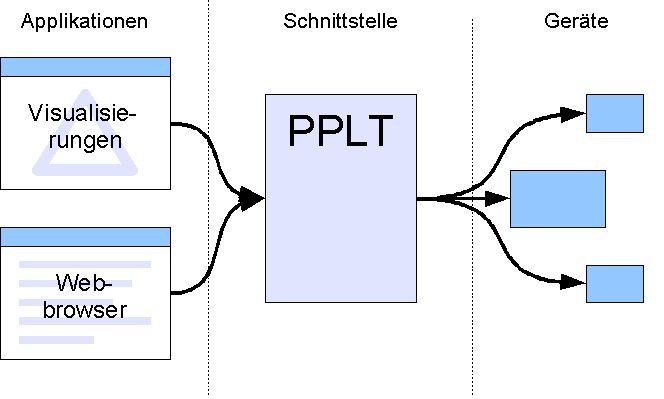
\includegraphics[scale=0.5]{ZieleGrenzen01}
		\caption{PPLT als Schnitstelle zwischen Applikationen und Ger�ten.}
		\label{fig:WiPPLT1}
	\end{figure}
	
	An einer solchen Position, ist es durchaus sinnvoll eine M�glchkeit zu haben
	zu bestimmen, wer auf welche Ger�te wie zugreifen darf. Daf�r wird ein so 
	genanntes Rechtemanagement ben�tigt. Solch eine \index{Rechteverwaltung}
	Rechteverwaltung bietet die PPLT. Sie besteht aus einer eigenen 
	\index{Benutzerdatenbank} Benutzerdatenbank, in der die \index{Benutzer} 
	Benutzer in hieraischen \index{Gruppen} Gruppen organisiert sind. 
	Zur \index{Authentifizierung} Authentifizierung des einzelnen	Benutzers 
	sind dann Benutzername und ein \index{Kennwort} Kennwort n�tig. Auf diese 
	Weise l�sst sich der Zugriff auf die Ger�te regeln, indem einzelnen 
	Benutztern	oder ganzen Gruppen der Zugriff auf Ger�te explizit gew�hrt 
	oder verboten wird.
	
	Dazu ein Beispiel:\\
	In einem Unternehmen sind die R�ume klimatisiert. Die Klimaanlage als
	automatisierter Prozess soll von den Mitarbeitern moduliert werden k�nnen.
	Um zu verhindern, dass ein Mitarbeiter aus Versehen oder Absicht die 
	Klimanalage eines Fremden B�ros manipuliert, sollte jeder Mitarbeiter nur
	Zugriff auf die Klimaanlage seines eigenen B�ros haben. 
	
	Um mit m�g\-lichst viele verschiedenen Programmen zusammen arbeiten zu k�n\-nen,
	besitzt die PPLT die M�glichkeit, die Schnittstelle zu den Applikationen 
	auszutauschen. Diese Schnittstelle wird hier \textit{Server} genannt. 
	\index{Server}Server sind im Allgemeinen Programme, die ihre Dienste anderen 
	Programmen zur Verf�gung stellen. So kann also die Unterst�tzung f�r ein 
	bestimmtes Programm, w�rend der Laufzeit in die PPLT geladen	werden.
	
	Dazu ein Beispiel:
	M�chte man von unterwegs mit dem PDA/Handy oder im Internet-Cafe �berpr�fen,
	ob man vieleicht zu Hause bestimmte Ger�te versehentlich nicht ausgeschaltet
	hat, so empfiehlt sich die Steuerung der Haushaltsger�te mittels Webserver,
	da sich ein Webbrowser mittlerweile auf jedem Handy finden l�sst. Also
	wird ein Webserver in die PPLT geladen, �ber den man sp�ter, nach einer
	Authentifikation\footnote{Login}, die Haushaltsger�te, zur Not von �berall aus,
	abschalten kann.

	\subsection{Grenzen}
	Die PPLT unterliegt wie jedes Programm bestimmten Grenzen. Anhand dieser kann
	man erkennen wo sich die Software einsetzten l�sst oder viel mehr, wo diese 
	nicht	verwendbar ist.
	
	Die PPLT l�sst sich grunds�tzlich nur als Master innerhalb eines Buses ein
	setzten. Diese Restriktion gild aber nur f�r die Kommunikation mit den 
	Gr�ten. Die PPLT kann also keine Anfrage eines Ger�tes verabeiten und
	Beantworten. Anfragen, die an einen Server der PPLT gestellt werden,
	kann das System aber sehr wohl bearbeiten. 
	
	Diese unscheinbar wirkende Einschr�nkung hat jedoch gro�e Auswirkungen
	auf das Einsatztgebiet der PPLT. So l�sst sich das System nur bedingt
	in der industriellen Produktion verwenden. Das Hauptproblem bei der 
	�berwachung solcher Prozesse liegt in der Reaktionszeit. Die PPLT
	m�sste zur �berwachung eines Prozesses dessen Werte zyklisch abfragen.
	Dabei kommt es aber zu unn�tig hohem Datenverkehr, da die PPLT die 
	mei�te Zeit sich nicht �nderne Werte sammelt und so ggf. auf ein
	Erreignis zu sp�t reagieren k�nnte. Die PPLT ist also f�r das 
	Monitoring von Prozessen nur eigeschr�nkt nutzbar.
	
	Die St�rke der PPLT liegt, bedingt durch ihre Konstruktion, in der
	aktiven Rolle\footnote{Also nicht in der passiven �berwachung.}.
	Also zum Beispiel in der Modulierung\footnote{Manipulation} 
	automatisierter Prozesse.
	

	\section{Technische Details}
\begin{itemize}
	\item PPLT vs pyDCPU
	\item Schalenmodell
	\item wozu es benutzt werden kann
	\item Grenzen (Nur Master im BUS, kein Multimaster-Betrieb, Polling)
	\item module schachtelbar, eigene Benutzerverwaltung, nicht be\-schr�nkt auf
	eine applikation (visualisierung)
	\item Modularisierung (Kern-Module, Ger�te, Server)
\end{itemize}	



\chapter{Erste Schritte}
	\section{Was ben�tige ich?}
	Um die PPLT benutzen zu k�nnen, m�ssen eine Reihe Bedingungen erf�llt sein. Sie ben�tigen
	zu aller erst den Python-Interpreter, da die PPLT in dieser Scriptsprache geschrieben wurde.
	Diesen Interpreter ist quelloffene Software und kann kostenlos von der URL
	\href{http://www.python.org}{www.python.org} heruntergeladen werden. Sie ben�tigen 
	jedoch Python ab der Version \textbf{2.3.0}.
	
	Wenn sie die grafische Applikation PPLT-Center (\texttt{PPLTC}) verwenden wollen, ben�tigen sie
	die wxPython Bibliothek. Diese Bibliothek erm�glicht die platform�bergreifende Programmierung von
	grafischen Benutzterprogrammen. Diese ist ebenso wie Python eine Quelloffene Bibliothek, die sie
	von der URL \href{http://www.wxpython.org}{www.wxpython.org} herunterladen. Da sich die 
	API der Bibliothek ver\-�ndert hat, ben�tigen sie mindestens die recht aktuelle Version 
	\textbf{2.5.0}. Zu beachten ist, dass sie diese Bibliothek nicht ben�tigen, wenn sie die 
	Applikation \texttt{PPLTC} nicht verwenden m�chten.
	
	Wenn sie das Betriebssystem \textbf{Windows} von Microsoft verwenden, sollten sie auf jeden
	fall die Python-Bibliothek pywin32 herunterladen. Diese ist ebenso quelloffen und ist unter
	der URL \href{http://pywin32.sourceforge.net}{pywin32.sourceforge.net} herunterladen. 
	Dieses Projekt verfolgt eine recht eigensinnige Versionsnummerierung. Die ben�tigen 
	mindestens die Version \textbf{203}. Wenn sie jedoch	\textbf{Posix} 
	kompatible\footnote{Linux, Unix, HP-UX, BSD, ...} Betriebssysteme verwenden,
	ben�tigen sie diese Bibliothek nicht.
	
	Es kann durchaus vorkommen, dass ein bestimmtes Kern-Modul eine weitere, nicht in der Standard
	Bibliothek enthaltene, Bibliothek ben�tigt. Dies entnehmen sie bitte der der Dokumentation des
	einzelnen Moduls. Ich einieger Voraussicht laden sie bitte die Bibliothek
	pyserial von der URL \href{http://pyserial.sourceforge.net}{pyserial.sourceforge.net}
	herunter. Diese Bibliothek bietet eine Platform\-�bergreifende M�glichkeit die serielle 
	Schnitstelle zu nutzen. Diese Bibliothek wird von der Kern-Bibliothek \texttt{UniSerial} 
	verwendet, welches selber	wieder von einer Vielzahl von Ger�ten verwendet wird.
	
	An dieser Stelle m�chte ich anmerken, dass f�r die ersten Versuche mit der PPLT keinerlei
	besondere Hardware von N�ten ist. Dementsprechend sind die Beispiele aber etwas 
	unspektakul�r. Sie beschr�nken sich auf das erzeugen von Zufallswerten.

	\subsection{Installation der Software}
	Ich kann ihnen an dieser Stelle keine vollst�ndige Installationsanleitung
	f�r diese Pakete anbieten. Dies w�rde den Rahmen dieses Dokumentes Spr�ngen.
	
	Dennoch will ich ihnen hier eine kurze "`Schritt f�r Schritt"'-Anleitung 
	zur Installation geben. Die Installation der PPLT wird im n�chsten Abschnitt 
	besprochen.
	
	\subsubsection{Unter Windows}
		Die Installation von Python, wxPython und der pywin32 Erweiterung d�rfte sich 
		unter Windows recht	Problemlos gestalten. F�r all diese Pakete gibt es so
		gennte Installer. Dies sind ausf�hrbare Dateien\footnote{Unter Windows *.exe},
		die den Installationsprozess automatisieren. Nach dem Starten eines solchen
		Installers �ffnet sich ein Dialog, der die f�r die Installation ben�tigten
		Eingaben abfragt. Mei�t k�nnen sie die dort stehenden Standard Werte �bernehmen.
		
		Bei der Installation von Python wird am Anfang das Verzeichnis abgefragt, in
		das Python installiert werden soll. (Siehe Abbildung \ref{fig:PyInstall})
		Bitte merken oder notieren sie sich dieses Verzeichnis, es wird sp�ter 
		ben�tigt um die Dateien der PPLT wieder zu finden. 

		\begin{figure}[ht]
			\centering
			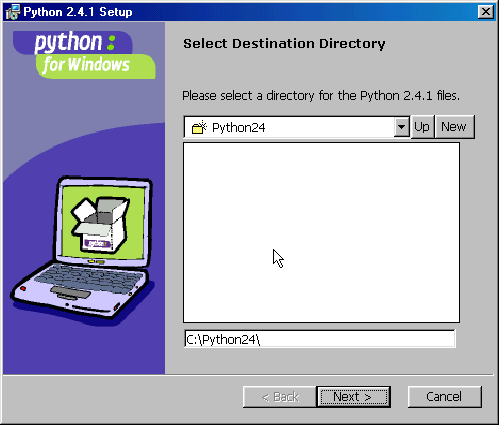
\includegraphics[scale=0.5]{PythonInstall}
			\caption{Python Installer}
			\label{fig:PyInstall}
		\end{figure}
		
		In diesem Verzeichnis	liegt auch die ausf�hrbare Datei des Python-Interpreters. 
		Bitte �ffnen sie jetzt eine Eingabeaufforderung und geben sie \texttt{python}
		ein. Nun sollte sich die Python-Konsolle �ffnen\footnote{Mit Strg-Z beenden die
		die Konsole}. Ist dies nicht der Fall und sie erhalten einen Fehler, dass
		dieser Befehl unbekannt sei, m�ssen sie Windows mitteilen, dass es auch in 
		dem oben erw�hnten Verzeichnis nach ausf�hrbaren Dateien suchen soll.
		
		Dies k�nnen sie unter Windows95/98 mit einem Text-Editor oder dem Programm
		\texttt{msconfig} erledigen. Editiren sie die 
		\texttt{autoexec.bat}\footnote{Mei�t dierekt auf dem Laufwerk \texttt{C:}}
		und f�gen sie die Zeile \texttt{set PATH=\%PATH\%;C:$\backslash$Python24$\backslash$} 
		hinzu\footnote{Bitte ersetzen sie C:$\backslash$Python24$\backslash$ mit dem Verzeichnis, in das
		sie Python installiert haben.}.
		
		Unter Windows 2000/XP gestaltet sich dieser Eintrag einfacher. �ffnen sie
		bitte \texttt{Systemsteuerung->System}\footnote{Bitte beachten sie, dass sie unter
		Windows 2000/XP als Systemadministrator angemeldet seien m�ssen}. W�hlen sie den Reiter 
		\texttt{Erweitert} aus und klicken sie auf \texttt{Umgebungsvariablen}.
		Es �ffnet sich ein Fenster indem sie die Umgebungsvariablen f�r den 
		aktuellen Benutzer und das System setzen k�nnen. Unter den Systemvariablen
		befindet sich auch die Variable \texttt{Path}. W�hlen sie diese aus und
		klicken sie auf \texttt{Bearbeiten}. F�gen sie bei \texttt{Wert der Variablen}
		\texttt{;C:$\backslash$Python24$\backslash$} hinzu, oder eben das Verzeichnis, in das sie Python
		installiert haben.
		
		Bitte beachten sie das Semikolon. Wird dieses vergessen, kann das das Verhalten
		anderer Programme beeinflussen.
		
		Bitte beachten sie, dass sie \textbf{zuerst} Python und \textbf{dann} 
		wxPython und pywin32 installieren.
		
		Die Installation von pyserial k�nnte sich etwas schwierieger gestalten, da
		f�r dieses Packet nicht unbedingt ein Installer vorliegt. Ist dies nicht der
		Fall, laden sie bitte das Quellarchiv herunter und entpacken es. 
		
		Starten sie dann eine Konsole\footnote{MS-DOS Eingabeaufforderung} und
		wechseln sie mit \texttt{cd} in das Verzeichnis, das sie entpackt haben.
		
		F�hren sie nun \texttt{python setup.py install} aus\footnote{Achten sie bitte auf
		die Leerzeichen}. Nun sollte die Bibliothek installiert werden. 
		
	\subsubsection{Unter Posix}
		Die Installation der Software unter Posix-Systemen wie Linux, Unix oder BSD gestaltet sich 
		von Anbieter zu Anbieter recht unterschiedlich. Am einfachsten ist es, wenn der Distributor
		die ben�tigte Software als Inastallationspakete\footnote{Zum Beispiel als RPM oder DEB Dateien} 
		im Bin�rformat anbietet. Python und wxPython werden bei den gro�en Distributionen mitgelifert.
		Aktuelle Distributionen d�rften auch die neueren Pakete, also in der aktuellen Version, enthalten.
		Jedoch ist in der SuSE 9.1 Distribution eine zu alte Version von wxPython enthalten, so dass diese
		aktualisiert werden sollte.
		
		Am sichersten sind sie, wenn sie die Quellen von Python sowie wxPython heunterladen und
		selber kompalieren. Dies sei aber nur erfahreren Benutzern empfohlen.
		
		F�r die Linux Distributionen Debian und Red Head liegen auch fertige Bin�r-Installationspackete
		auf dem Servern von Python und wxPython. Diese sollten sich mit dem Paketmanager der jeweiligen
		Distribution problemlos installieren lassen.
		
		Zur installation den pyserial Bibliothek empfiehlt es sich die Quellen\footnote{Mit der Endung 
		\texttt{tar.gz} oder \texttt{tar.bz2}} herunter zu laden. Dieses Archiv enth�lt ein 
		Installationsscript, mit dessen Hilfe die Installation sehr einfach durchgef�hrt werden kann.
		
		Wechseln sie auf eine Konsole und gehen sie in das Verzeichnis, indas sie das Archiv gespeichert haben.
		Entpacken sie das Archiv mit: 
		
		\texttt{tar -x?? pyserial-???.tar.gz} 
		
		Es sollte nun ein neues
		Verzeichnis mit dem Namen \texttt{pyserial-???} im aktuellen erzeugtworden sein. Wechseln sie
		in dieses Verzeichnis und f�hren sie:
		
		\texttt{python setup.py install} aus.
		 
		Nun wird die Bibliothek installiert.
		
		Sind alle erw�hnten Softwarepakete installiert, k�nnen sie mit der Installation der PPLT
		beginnen. Sollten bei der Installation Probleme auf treten oder wenn sie Fragen zu diesem
		Text haben, wenden sie sich bitte per E-Mail an mich.
		
	\section{PPLT Installieren}
	\subsection{PPLT Center}



\end{document}
